
\section{Differentialgleichungen erster Ordnung}

\subsection{Eine graphische Lösungsmethode: Richtungsfelder}

Betrachten wir als Beispiel die Differentialgleichung
\[
    \dot{x}(t)=1+t-x(t).
\]

Angenommen, wir suchen eine Lösung \(x(t)\) mit der Eigenschaft,
dass \(x(2)=1\) gilt. Was wissen wir über den Graphen von
\(x(t)\) im \(tx\)-Diagramm? Er verläuft durch den Punkt
\(P(2|1)\) und die Tangente hat an dieser Stelle die Steigung:
\(\dot{x}(2)=1+2-1=2\).

Etwas allgemeiner: Wenn der Graph der Lösung durch den Punkt
\(P(t_0|x_0)\) verläuft, dann hat er an dieser Stelle eine
Tangente mit der Steigung
\[
    m=1+t_0-x_0.
\]

\begin{LA}{Einführungsaufgabe: Richtungsfelder}{LA:richtungsfelder}

    Berechnen Sie einige Steigungen in Abhängigkeit von \(t\)
    und \(x\) und tragen Sie sie in die Grafik ein.

    % \begin{center}
    %     \begin{tikzpicture}[
    %             scale=0.82,
    %             every node/.style={font=\small}
    %         ]
    %         % Tabelle links
    %         \begin{scope}[shift={(-8.7,0)}]

    %             % Kopfzeile
    %             \fill[blue!25] (0,4) rectangle (8,4.7);

    %             % Zeilenbeschriftungen
    %             \fill[blue!25] (0,0.5) rectangle (1,4);

    %             % Hintergrund der Datenfelder
    %             \fill[gray!25] (1,0.5) rectangle (8,4);

    %             % Vertikale Gitterlinien
    %             \foreach \i in {0,...,8} {
    %                     \draw[black!30,thin]
    %                     (\i,0.5) -- (\i,4.7);
    %                 }

    %             % Horizontale Gitterlinien
    %             \foreach \j in {0,...,6} {
    %                     \draw[black!30,thin]
    %                     (0,{0.5+0.7*\j}) -- (8,{0.5+0.7*\j});
    %                 }
    %             % Kopfzeile
    %             \node[text=white,font=\bfseries]
    %             at (0.5,4.35) {\(x\backslash t\)};

    %             \foreach \t [count=\i from 1] in {-3,-2,-1,0,1,2,3} {
    %                     \node[text=white,font=\bfseries]
    %                     at (\i+0.5,4.35) {\(\t\)};
    %                 }

    %             % Zeilenbeschriftungen
    %             \foreach \x [count=\j from 0] in {2,1,0,-1,-2} {
    %                     \node[text=white,font=\bfseries]
    %                     at (0.5,{3.65-0.7*\j}) {\(\x\)};
    %                 }

    %             % Vorgegebener Wert: t=2, x=1
    %             \node at (6.5,2.95) {\(2\)};
    %         \end{scope}

    %         % Koordinatensystem rechts
    %         \begin{scope}[shift={(3.5,2.35)},scale=0.9]
    %             % Gestricheltes Gitternetz
    %             \draw[
    %                 gray!60,
    %                 dashed,
    %                 line width=0.5pt
    %             ] (-3.5,-2.35) grid (3.5,2.35);

    %             % Achsen
    %             \draw[->,thick]
    %             (-3.5,0) -- (3.75,0)
    %             node[below] {\(t\)};

    %             \draw[->,thick]
    %             (0,-2.35) -- (0,2.55)
    %             node[right] {\(x\)};

    %             % Achsenbeschriftungen
    %             \foreach \t in {-3,-2,-1,1,2,3} {
    %                     \node[below,font=\scriptsize]
    %                     at (\t,0) {\(\t\)};
    %                 }

    %             \foreach \x in {-2,-1,1,2} {
    %                     \node[left,font=\scriptsize]
    %                     at (0,\x) {\(\x\)};
    %                 }

    %             \node[below left,font=\scriptsize]
    %             at (0,0) {\(0\)};

    %             % Vorgegebenes Steigungsstück bei (2,1)
    %             % Steigung m = 1+2-1 = 2
    %             \draw[very thick]
    %             (1.88,0.76) -- (2.12,1.24);
    %         \end{scope}
    %     \end{tikzpicture}
    % \end{center}



    % Tabelle
    \begin{center}
        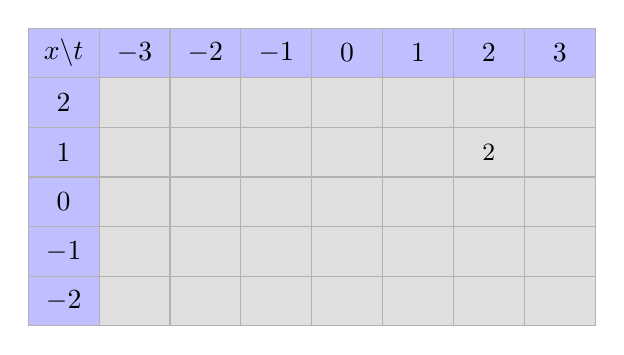
\begin{tikzpicture}[
                scale=0.9,
                every node/.style={font=\small}
            ]
            % Kopfzeile
            \fill[blue!25] (0,4) rectangle (8,4.7);

            % Zeilenbeschriftungen
            \fill[blue!25] (0,0.5) rectangle (1,4);

            % Hintergrund der Datenfelder
            \fill[gray!25] (1,0.5) rectangle (8,4);

            % Vertikale Gitterlinien
            \foreach \i in {0,...,8} {
                    \draw[black!30,thin]
                    (\i,0.5) -- (\i,4.7);
                }

            % Horizontale Gitterlinien
            \foreach \j in {0,...,6} {
                    \draw[black!30,thin]
                    (0,{0.5+0.7*\j}) -- (8,{0.5+0.7*\j});
                }

            % Kopfzeile
            \node[font=\bfseries]
            at (0.5,4.35) {\(x\backslash t\)};

            \foreach \t [count=\i from 1] in {-3,-2,-1,0,1,2,3} {
                    \node[font=\bfseries]
                    at (\i+0.5,4.35) {\(\t\)};
                }

            % Zeilenbeschriftungen
            \foreach \x [count=\j from 0] in {2,1,0,-1,-2} {
                    \node[font=\bfseries]
                    at (0.5,{3.65-0.7*\j}) {\(\x\)};
                }

            % Vorgegebener Wert
            \node at (6.5,2.95) {\(2\)};
        \end{tikzpicture}
    \end{center}

    % Koordinatensystem
    \begin{center}
        \begin{tikzpicture}[
                scale=1.5,
                every node/.style={font=\small}
            ]
            % Gestricheltes Gitternetz
            \draw[
                gray!60,
                dashed,
                line width=0.4pt
            ] (-3.5,-2.5) grid (3.5,2.5);

            % Achsen
            \draw[->,thick]
            (-3.5,0) -- (3.75,0)
            node[below] {\(t\)};

            \draw[->,thick]
            (0,-2.5) -- (0,2.75)
            node[right] {\(x\)};

            % Achsenbeschriftungen
            \foreach \t in {-3,-2,-1,1,2,3} {
                    \node[below,font=\scriptsize]
                    at (\t,0) {\(\t\)};
                }

            \foreach \x in {-2,-1,1,2} {
                    \node[left,font=\scriptsize]
                    at (0,\x) {\(\x\)};
                }

            \node[below left,font=\scriptsize]
            at (0,0) {\(0\)};

            % Vorgegebenes Steigungsstück bei (2,1)
            % Steigung m = 2
            \draw[very thick]
            (1.88,0.76) -- (2.12,1.24);

        \end{tikzpicture}
    \end{center}

    Schätzen Sie, wie die Lösungskurven verlaufen, wenn
    die Anfangsbedingung

    \begin{enumerate}
        \item \(x(0)=1\),
        \item \(x(0)=0\) oder
        \item \(x(0)=-2\)
    \end{enumerate}

    lautet.

\end{LA}

\clearpage

Einen qualitativen Eindruck über die Lösungen von Differentialgleichungen
kann man mit sogenannten \textbf{Richtungsfeldern} erhalten.
Das folgende Bild zeigt ein solches Richtungsfeld für die
Differentialgleichung
\[
    \dot{x}(t)=1+\frac{x(t)}{t}.
\]
Zusätzlich ist eine Lösung zur Anfangsbedingung \(x(1)=0\)
eingezeichnet.
\begin{center}
    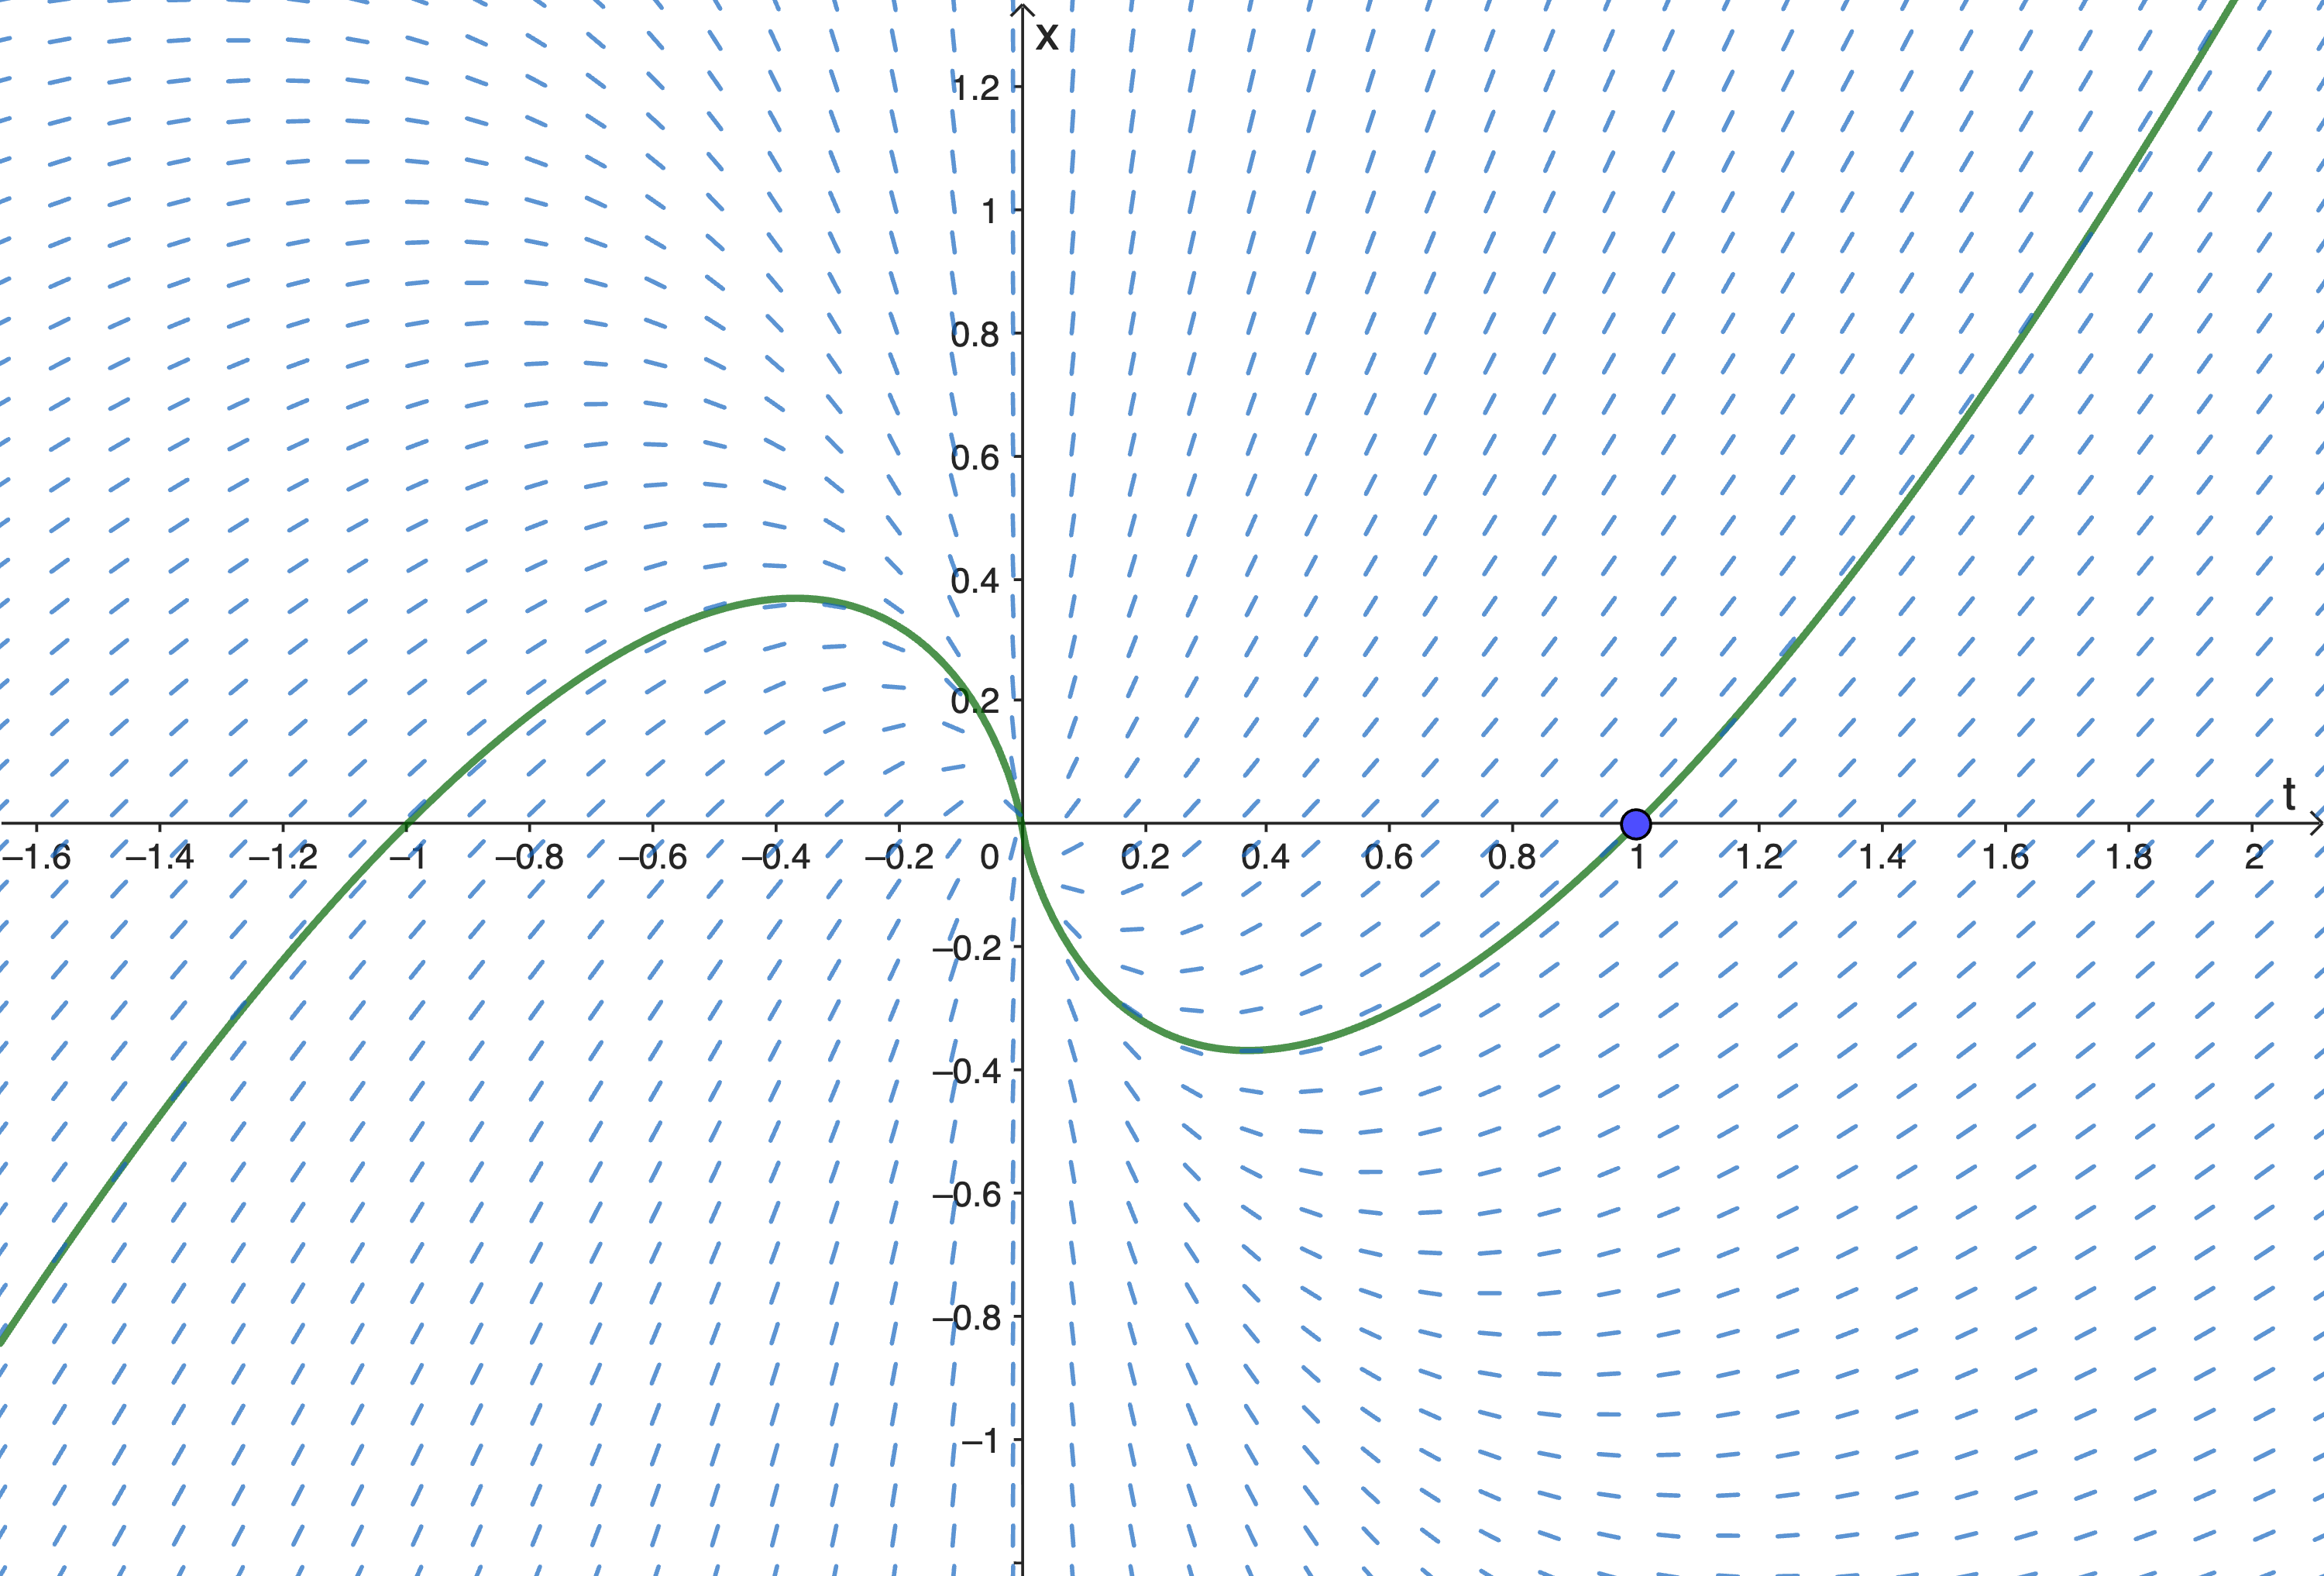
\includegraphics[width = 0.5\textwidth]{media/richtungsfeld-bsp.png}
\end{center}

% \begin{center}
%     \begin{tikzpicture}[scale=0.95,>=stealth]
%         % Richtungsfeld

%         % Richtungsfeld

%         \begin{scope}
%             \clip (-3.2,-3.2) rectangle (3.2,3.2);

%             \foreach \x in {-3,-2.7,...,-0.3,0.3,0.6,...,3} {
%                     \foreach \y in {-3,-2.7,...,3} {

%                             % Steigung
%                             \pgfmathsetmacro{\m}{1+\y/\x}

%                             % Normierter Richtungsvektor
%                             \pgfmathsetmacro{\dx}{0.12/sqrt(1+\m*\m)}
%                             \pgfmathsetmacro{\dy}{\m*\dx}

%                             % Steigungsstück
%                             \draw[blue,thin]
%                             ({\x-\dx},{\y-\dy}) --
%                             ({\x+\dx},{\y+\dy});
%                         }
%                 }
%         \end{scope}


%         % Achsen
%         \draw[->,thick] (-3.4,0) -- (3.5,0)
%         node[right] {\(x\)};
%         \draw[->,thick] (0,-3.4) -- (0,3.5)
%         node[above] {\(y\)};

%         % Achsenbeschriftungen
%         \foreach \i in {-3,-2,-1,1,2,3} {
%                 \draw (\i,0.05) -- (\i,-0.05);
%                 \node[below,font=\scriptsize] at (\i,0) {\(\i\)};
%                 \draw (0.05,\i) -- (-0.05,\i);
%                 \node[left,font=\scriptsize] at (0,\i) {\(\i\)};
%             }

%         % Anfangspunkt
%         \fill[red] (0,0) circle (1.2pt);
%     \end{tikzpicture}
% \end{center}

Eine effiziente Methode, solche Richtungsfelder zu erstellen,
ist das sogenannte \textbf{Isoklinen-Verfahren}.
Eine Isokline einer Differentialgleichung erster Ordnung ist
eine Kurve, auf der die erste Ableitung konstant ist.
Sämtliche Lösungskurven schneiden also eine Isokline
unter demselben Winkel.

\begin{bsp}{Isoklinen}{bsp:isoklinen}
    Betrachten wir die Differentialgleichung
    \[
        \dot{x}(t)=x(t)-t.
    \]
    Auf der Isokline zur Steigung \(k\) ist die erste Ableitung
    konstant gleich \(k\), also gilt
    \[
        k=x-t
        \qquad\Longleftrightarrow\qquad
        x=t+k.
    \]


    \begin{center}
        \begin{tikzpicture}[
                scale=1.35,
                every node/.style={font=\small},
                >=stealth
            ]
            % Gestricheltes Gitternetz
            \draw[
                gray!55,
                dashed,
                line width=0.5pt
            ] (-2.7,-2.4) grid (3.7,3.4);

            % Achsen
            \draw[->,thick]
            (-2.7,0) -- (3.9,0)
            node[above] {\(t\)};

            \draw[->,thick]
            (0,-2.4) -- (0,3.6)
            node[right] {\(x\)};

            % Beschriftungen
            \foreach \t in {-2,-1,1,2,3} {
                    \node[below,font=\scriptsize]
                    at (\t,0) {\(\t\)};
                }

            \foreach \x in {-2,-1,1,2,3} {
                    \node[left,font=\scriptsize]
                    at (0,\x) {\(\x\)};
                }

            \node[below right,font=\scriptsize]
            at (0,0) {\(0\)};
        \end{tikzpicture}
    \end{center}
\end{bsp}
\begin{ueb}{Richtungsfelder skizzieren}{ueb:richtungsfelder_skizzieren}
    Skizzieren Sie das Richtungsfeld der Differentialgleichung
    und zeichnen Sie nach Augenmass eine Lösungskurve.

    Was könnte es für eine Kurve sein?
    Überprüfen Sie Ihre Vermutung durch Einsetzen in die
    Differentialgleichung.

    \begin{enumerate}
        \item \(\dot{x}(t)=t\)
        \item \(\dot{x}(t)\cdot t=1\)
        \item \(\dot{x}(t)=x(t)\)
        \item \(\dot{x}(t)\cdot x(t)=1\)
        \item \(t\cdot\dot{x}(t)+x(t)=0\)
        \item \(\dot{x}(t)=t^2-t\)
    \end{enumerate}

    \textit{Tipp:} In \href{https://www.geogebra.org/calculator}{GeoGebra} kann man mit dem Befehl
    \texttt{Richtungsfeld} solche Felder zeichnen lassen.
    Damit können Sie Ihre Lösungen kontrollieren.
    Beachten Sie aber, dass die gesuchte Funktion mit \(y\)
    und die unabhängige Variable mit \(x\) bezeichnet
    werden muss.
\end{ueb}































\clearpage

\subsection{Eine numerische Lösungsmethode: Das Eulerverfahren}

So vielfältig die Anwendungen sind, die auf Differentialgleichungen
führen, so schwierig ist es im Einzelnen, eine Lösung zu bestimmen.
Die meisten Differentialgleichungen lassen sich gar nicht exakt lösen.
In solchen Fällen ist man auf Verfahren angewiesen, die es
ermöglichen, wenigstens einen approximativen Verlauf der
Lösungsfunktion anzugeben.

Ein solches Verfahren haben wir bereits kennengelernt.
Mithilfe von Richtungsfeldern kann man einen ungefähren Verlauf
der Lösungskurve angeben\footnote{Diese Verfahren sind gar nicht so schlecht. Die Bahn der Sonde InSight, die 2019 auf dem Mars gelandet ist, wurde mit
    solchen Verfahren berechnet. Die Landezone hatte etwa die Grösse eines Fussballfelds und war von der Erde ungefähr 228
    Millionen Kilometer entfernt!}.

Zeichnen Sie im folgenden Richtungsfeld zur Differentialgleichung
\[
    \dot{x}(t)=x(t)-2t
\]
den Verlauf der Lösungskurve mit der Anfangsbedingung \(x(0)=0.5\).

\begin{center}
    \begin{tikzpicture}[
            x=8cm,
            y=8cm,
            >=stealth
        ]
        % Begrenzung des Richtungsfeldes
        \begin{scope}
            \clip (-0.27,-0.16) rectangle (1.33,1.10);

            % Gestricheltes Gitternetz
            \draw[
                gray!45,
                dashed,
                line width=0.4pt
            ] (-0.2,-0.15) grid[
                    xstep=0.2,
                    ystep=0.2
                ] (1.2,1.0);

            % Richtungsfeld: x'(t)=x(t)-2t
            \foreach \i in {-1,...,6} {
                    \foreach \j in {-1,...,5} {
                            \pgfmathsetmacro{\t}{0.2*\i}
                            \pgfmathsetmacro{\xx}{0.2*\j}

                            % Steigung
                            \pgfmathsetmacro{\m}{\xx-2*\t}

                            % Normierter Richtungsvektor
                            \pgfmathsetmacro{\dx}{0.032/sqrt(1+\m*\m)}
                            \pgfmathsetmacro{\dy}{\m*\dx}

                            % Steigungsstück
                            \draw[black,thin]
                            ({\t-\dx},{\xx-\dy}) --
                            ({\t+\dx},{\xx+\dy});
                        }
                }
        \end{scope}

        % Koordinatenachsen
        \draw[->,thick]
        (-0.27,0) -- (1.33,0)
        node[below] {\(t\)};

        \draw[->,thick]
        (0,-0.16) -- (0,1.10)
        node[above] {\(x\)};

        % Beschriftung der t-Achse
        \foreach \i in {-1,1,...,6} {
                \pgfmathsetmacro{\t}{0.2*\i}
                \draw (\t,0.008) -- (\t,-0.008);
                \node[below,font=\scriptsize]
                at (\t,-0.015)
                {\pgfmathprintnumber[fixed,precision=1]{\t}};
            }

        % Beschriftung der x-Achse
        \foreach \xx in {0.5,1} {
                \draw (0.008,\xx) -- (-0.008,\xx);
                \node[left,font=\scriptsize]
                at (-0.012,\xx)
                {\pgfmathprintnumber[fixed,precision=1]{\xx}};
            }

        \node[below right,font=\scriptsize]
        at (0,0) {\(0\)};

    \end{tikzpicture}
\end{center}

Das \textbf{Eulerverfahren} ist im Grunde eine numerische
Umsetzung der Idee der Richtungsfelder.
Das Einführungsbeispiel zu diesem Verfahren wird in der
Klasse behandelt.



\begin{bsp}{Einführungsbeispiel zum Eulerverfahren}{bsp:euler_einfuehrung}

    \textbf{Gegeben} ist das Anfangswertproblem
    \[
        \begin{cases}
            \dot{x}(t)=x(t)-2t, \\
            x(0)=0.5.
        \end{cases}
    \]
    \textbf{Gesucht} ist eine Schätzung für den Funktionswert \(x(1)\).

    \textbf{Idee:} Die Lösungskurve wird schrittweise durch
    Tangenten angenähert, beispielsweise mit der Schrittweite \(h=0.2\).

    \begin{center}
        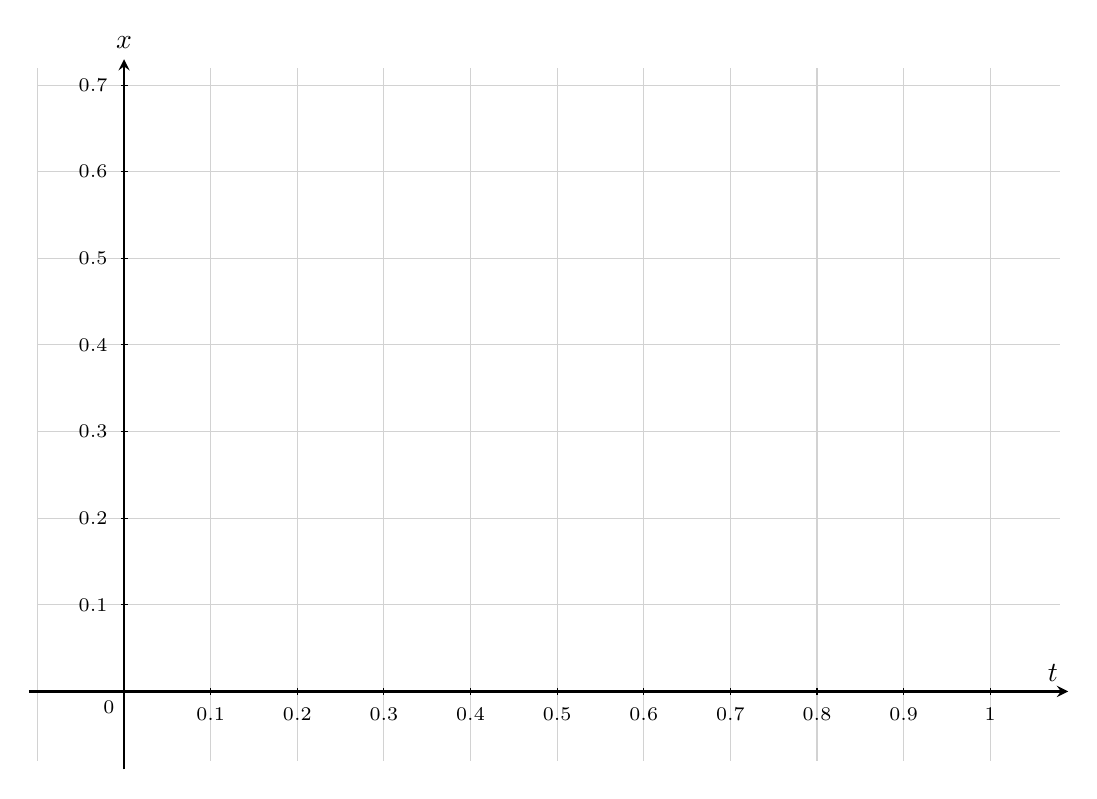
\begin{tikzpicture}[
                x=11cm,
                y=11cm,
                >=stealth
            ]
            % Zeichenbereich
            \begin{scope}
                \clip (-0.11,-0.09) rectangle (1.09,0.73);

                % Feines Gitternetz (Schrittweite 0.02)
                % \draw[
                %     gray!12,
                %     very thin,
                %     step=0.02
                % ] (-0.1,-0.08) grid (1.08,0.72);

                % Grobes Gitternetz (Schrittweite 0.1)
                \draw[
                    gray!35,
                    thin,
                    step=0.1
                ] (-0.1,-0.08) grid (1.08,0.72);
            \end{scope}

            % Koordinatenachsen
            \draw[->,thick]
            (-0.11,0) -- (1.09,0)
            node[above left] {\(t\)};

            \draw[->,thick]
            (0,-0.09) -- (0,0.73)
            node[above] {\(x\)};

            % Beschriftung der t-Achse
            \foreach \i in {1,...,10} {
                    \pgfmathsetmacro{\t}{0.1*\i}
                    \draw (\t,0.004) -- (\t,-0.004);
                    \node[below,font=\scriptsize]
                    at (\t,-0.008)
                    {\pgfmathprintnumber[fixed,precision=1]{\t}};
                }

            % Beschriftung der x-Achse
            \foreach \i in {1,...,7} {
                    \pgfmathsetmacro{\xx}{0.1*\i}
                    \draw (0.004,\xx) -- (-0.004,\xx);
                    \node[left,font=\scriptsize]
                    at (-0.008,\xx)
                    {\pgfmathprintnumber[fixed,precision=1]{\xx}};
                }

            \node[below left,font=\scriptsize]
            at (0,0) {\(0\)};

        \end{tikzpicture}
    \end{center}

    \begin{center}
        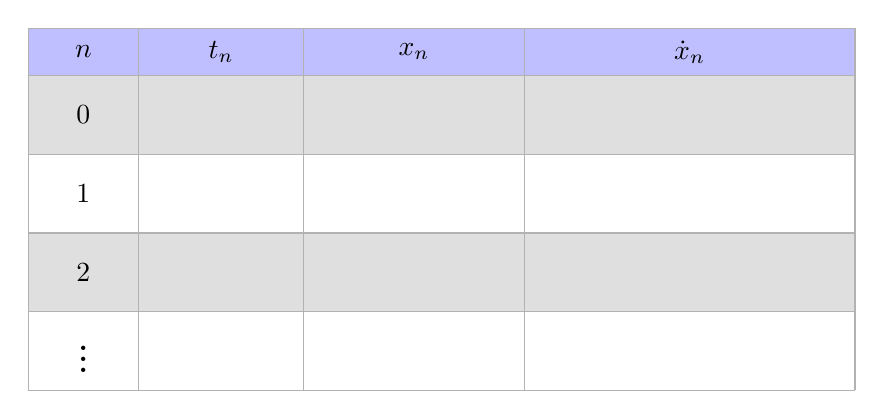
\begin{tikzpicture}[
                x=1.4cm,
                y=1cm,
                every node/.style={font=\small}
            ]
            % Spaltenbreiten:
            % n: 1, t_n: 1.5, x_n: 2, x'_n: 3
            % Gesamtbreite: 7.5

            % Kopfzeile
            \fill[blue!25]
            (0,5) rectangle (7.5,5.6);

            % Abwechselnd hinterlegte Datenzeilen
            \fill[gray!25]
            (0,4) rectangle (7.5,5);
            \fill[gray!25]
            (0,2) rectangle (7.5,3);

            % Vertikale Gitterlinien
            \foreach \x in {0,1,2.5,4.5,7.5} {
                    \draw[black!30,thin]
                    (\x,1) -- (\x,5.6);
                }

            % Horizontale Gitterlinien
            \foreach \y in {1,2,3,4,5,5.6} {
                    \draw[black!30,thin]
                    (0,\y) -- (7.5,\y);
                }

            % Kopfzeile
            \node[font=\bfseries] at (0.5,5.3) {\(n\)};
            \node[font=\bfseries] at (1.75,5.3) {\(t_n\)};
            \node[font=\bfseries] at (3.5,5.3) {\(x_n\)};
            \node[font=\bfseries] at (6,5.3) {\(\dot{x}_n\)};

            % Zeilennummern
            \node[font=\bfseries] at (0.5,4.5) {\(0\)};
            \node[font=\bfseries] at (0.5,3.5) {\(1\)};
            \node[font=\bfseries] at (0.5,2.5) {\(2\)};
            \node[font=\bfseries] at (0.5,1.5) {\(\vdots\)};

        \end{tikzpicture}
    \end{center}

\end{bsp}

\begin{ueb}{Das Eulerverfahren}{ueb:eulerverfahren}

    Für die folgenden Aufgaben stehen auf Moodle eine
    \textbf{Excel-Vorlage} und eine \textbf{Python-Vorlage}
    zur Verfügung. Sie können selbst wählen, mit welcher
    der beiden Vorlagen Sie arbeiten möchten.

    \begin{enumerate}
        \item Betrachten Sie die Differentialgleichung
              \(\dot{x}(t)=x(t)-2t\) aus dem Einführungsbeispiel.

              \begin{enumerate}
                  \item Untersuchen Sie die Vorlage und die darin vorkommenden Formeln.
                        Wie sind diese zu verstehen?

                  \item Erweitern Sie die Vorlage so, dass
                        weitere Schritte des Eulerverfahrens
                        berechnet werden können.

                  \item Berechnen Sie eine Approximation der
                        Lösungskurve mit der Schrittweite \(h=0.1\)
                        im Intervall \(t\in[0,1]\).

                  \item Berechnen Sie zusätzlich eine Approximation
                        mit der Schrittweite \(h=0.01\).
                        Speichern Sie beide Approximationen,
                        da Sie diese später noch benötigen.

                  \item Zeigen Sie durch Einsetzen in die
                        Differentialgleichung, dass die gesuchte
                        Funktion die Gleichung
                        \[
                            x(t)=-\frac{3}{2}e^t+2t+2
                        \]
                        hat.

                  \item Vergleichen Sie die beiden Approximationen
                        und die exakte Lösung an der Stelle \(t=1\).

                  \item Berechnen Sie eine Wertetabelle für die
                        exakte Lösung mit der Schrittweite \(h=0.1\)
                        im Intervall \(t\in[0,1]\).

                        \textit{Tipp:} In Excel berechnet
                        \texttt{EXP(x)} den Wert von \(e^x\).
                        In Python können Sie dazu
                        \texttt{math.exp(x)} verwenden.

                  \item Zeichnen Sie die Graphen der beiden
                        Approximationen und der exakten Lösung
                        in einem gemeinsamen Koordinatensystem.

                        Verwenden Sie in Excel ein
                        \enquote{Punkt XY}-Diagramm oder in Python
                        eine entsprechende grafische Darstellung.
              \end{enumerate}

        \item Betrachten Sie die Differentialgleichung
              \[
                  \dot{x}(t)=1+(x(t)-t)^2
              \]
              mit der Anfangsbedingung \(x(0)=0.5\).
              Verwenden Sie die Excel- oder Python-Vorlage
              zur Lösung der folgenden Aufgaben.

              \begin{enumerate}
                  \item Berechnen Sie eine Approximation der
                        Lösungskurve im Intervall \(t\in[0,1]\)

                        \begin{enumerate}[label=\roman*)]
                            \item mit der Schrittweite \(h=0.1\),
                            \item mit der Schrittweite \(h=0.01\).
                        \end{enumerate}

                  \item Weisen Sie nach, dass die Funktion
                        \[
                            x(t)=t+\frac{1}{2-t}
                        \]
                        die Differentialgleichung löst.

                  \item Vergleichen Sie die Approximationen und
                        die exakte Lösung an der Stelle \(t=1\).

                  \item Zeichnen Sie die beiden Approximationen
                        und die exakte Lösung in einem gemeinsamen
                        Koordinatensystem.
              \end{enumerate}

        \item Das Wachstum einer Population von Bakterien wird
              häufig mit einer Exponentialfunktion modelliert.
              Tatsächlich wachsen die Bakterien in einem Reagenzglas
              nicht unbeschränkt weiter. Sobald die Ressourcen
              Nahrung und Platz knapp werden, wird das Wachstum
              gebremst.

              Der holländische Biomathematiker Verhulst hat aus
              diesem Grund ein alternatives Modell vorgeschlagen.
              Beim sogenannten \textbf{logistischen Wachstumsmodell}
              erfüllt die Funktion \(p(t)\), welche die Anzahl
              Individuen zur Zeit \(t\) angibt, die
              Differentialgleichung
              \[
                  \dot{p}(t)=a\cdot p(t)-b\cdot p(t)^2.
              \]

              Wir untersuchen den Fall \(a=b=4\) mit der
              Anfangsbedingung \(p(0)=0.5\).

              \begin{enumerate}
                  \item Zeichnen Sie das Richtungsfeld für den
                        Fall \(a=b=4\) (von Hand oder mit GeoGebra).

                  \item Zeichnen Sie den Verlauf der Lösungskurve
                        in das Richtungsfeld. Schätzen Sie den
                        Grenzwert für \(t\to\infty\).

                  \item Berechnen Sie \textbf{ohne Excel oder Python}
                        eine Approximation für \(p(1)\) mit dem
                        Eulerverfahren und einer Schrittweite
                        von \(h=0.5\).

                  \item Berechnen Sie \textbf{mit Excel oder Python}
                        eine Approximation für \(p(1)\) mit dem
                        Eulerverfahren und einer Schrittweite
                        von \(h=0.01\).

                  \item Zeigen Sie, dass die Funktion
                        \[
                            p(t)=\frac{1}{1+e^{-4t}}
                        \]
                        die Differentialgleichung löst.
              \end{enumerate}
    \end{enumerate}

\end{ueb}
\clearpage

\begin{satz}{Das Eulerverfahren}{satz:eulerverfahren}

    \textbf{Gegeben:} Eine Differentialgleichung der Form
    \[
        \dot{x}(t)=f(t,x(t))
    \]
    mit Anfangsbedingung \(x(t_0)=x_0\).

    \textbf{Gesucht:} Ein approximativer Verlauf der Lösungskurve.

    \medskip
    \textbf{Verfahren:}

    Wählen Sie eine kleine Schrittweite \(h>0\) und betrachten
    Sie die Folge von Zeitpunkten
    \[
        t_n=t_0+nh,\qquad n=0,1,2,\ldots
    \]
    Bestimmen Sie rekursiv die Glieder der Folge
    \[
        \boxed{x_{n+1}=x_n+h\cdot f(t_n,x_n).}
    \]
    Die berechneten Werte \(x_n\) sind Approximationen
    der Werte \(x(t_n)\) der exakten Lösung des
    Anfangswertproblems.

    \begin{center}
        \begin{tikzpicture}[
                x=11cm,
                y=8cm,
                >=stealth
            ]
            % Achsen
            \draw[->,thick]
            (-0.05,0) -- (1.15,0)
            node[below] {\(t\)};

            \draw[->,thick]
            (0,-0.05) -- (0,0.85)
            node[above] {\(x\)};

            % Beschriftungen der t-Achse
            \foreach \i in {0,...,5} {
                    \pgfmathsetmacro{\t}{0.2*\i}
                    \draw (\t,0.005) -- (\t,-0.005);
                    \node[below,font=\scriptsize]
                    at (\t,-0.01)
                    {\pgfmathprintnumber[fixed,precision=1]{\t}};
                }

            % Beschriftungen der x-Achse
            \foreach \i in {1,...,4} {
                    \pgfmathsetmacro{\xx}{0.2*\i}
                    \draw (0.005,\xx) -- (-0.005,\xx);
                    \node[left,font=\scriptsize]
                    at (-0.01,\xx)
                    {\pgfmathprintnumber[fixed,precision=1]{\xx}};
                }

            % Euler-Approximation mit h=0.2
            % x'(t)=x(t)-2t, x(0)=0.5
            \draw[thick,gray!70]
            (0,0.5) --
            (0.2,0.6) --
            (0.4,0.64) --
            (0.6,0.608) --
            (0.8,0.4896) --
            (1,0.26752);

            % Euler-Stützpunkte
            \foreach \t/\xx in {
                    0/0.5,
                    0.2/0.6,
                    0.4/0.64,
                    0.6/0.608,
                    0.8/0.4896,
                    1/0.26752
                } {
                    \fill[blue] (\t,\xx) circle (1.5pt);
                }

        \end{tikzpicture}
    \end{center}

\end{satz}
























\clearpage
\subsection{Die Separation der Variablen}

Während wir mit dem Eulerverfahren eine Methode kennengelernt haben,
mit der man die Lösung einer Differentialgleichung \textbf{approximativ}
bestimmen kann, wollen wir nun Techniken kennenlernen, mit denen wir
bei einigen Differentialgleichungen die Funktionsgleichung der Lösung
bestimmen können.

\subsubsection{Die Substitutionsmethode der Integralrechnung}

Für die erste Lösungsmethode benötigen wir zunächst eine
Integrationstechnik: die Substitutionsregel.
Diese Integrationsmethode ist gewissermassen die Kettenregel
der Ableitung -- aber \enquote{rückwärts} angewendet!

Betrachten wir zunächst die andere Richtung: die Ableitung.
Sei \(F(x)\) eine Stammfunktion von \(f(x)\).
Dann gilt nach der Kettenregel:
\[
    \bigl(F(u(x))\bigr)'=f(u(x))\cdot u'(x).
\]
Das lässt sich auch so formulieren:

\begin{satz}{Substitutionsmethode}{satz:substitution}
    Sei \(F(t)\) eine Stammfunktion von \(f(t)\).
    Dann gilt
    \[
        \int f(u(t))\cdot u'(t)\,dt
        =F(u(t))+C.
    \]
\end{satz}

Diesen Satz kann man sich gut merken, wenn man die Schreibweise
\(\frac{d}{dt}\) für die Ableitung nach \(t\) verwendet:

\begin{satz}{Substitutionsmethode -- Kurzform}{satz:substitution_kurz}
    \[
        \int f(u)\frac{du}{dt}\,dt
        =\int f(u)\,du.
    \]
\end{satz}

So wird deutlich, woher der Name \enquote{Substitution} kommt:
Links wird nach der Variablen \(t\), rechts nach \(u\) integriert.
Man ersetzt (substituiert) die Variable, nach der integriert wird.

Die Schwierigkeit in der Anwendung besteht darin, die Funktionen
\(f(u)\) und \(u(t)\) zu erkennen.
Betrachten Sie das folgende Beispiel.

\begin{bsp}{Integration durch Substitution}{bsp:substitution}
    Berechnen Sie das Integral
    \[
        \int \frac{1-t}{\sqrt{2t-t^2}}\,dt.
    \]
    \karofeld{5}
\end{bsp}


\begin{ueb}{Integration durch Substitution}{ueb:substitution}

    Integrieren Sie die folgenden Funktionen.
    Überprüfen Sie das Resultat durch Ableiten.

    \begin{enumerate}[label=\alph*)]
        \item \(f(t)=\sqrt{t^3+1}\cdot 3t^2\)

        \item \(f(t)=\sin(t^2)\cdot t\)

        \item \(f(t)=\dfrac{t}{t^2+1}\)

        \item \(f(t)=(3t+5)^6\)

        \item \(f(t)=t\cdot(t^2+3)^{-4}\)

        \item \(f(t)=\dfrac{t^2}{\sqrt{4-t^3}}\)

        \item \(f(t)=\dfrac{\ln t}{t}\)

        \item \(f(t)=t\cdot e^{-t^2}\)

        \item \(f(t)=\dfrac{\sin(t)}{\cos(t)}\)

        \item \(f(t)=\dfrac{(\ln t)^4}{t}\)

        \item \textbf{Challenge:}
              \(f(t)=t^3(t+1)^3(2t+1)\)
    \end{enumerate}

\end{ueb}


















\clearpage


\subsubsection{Die Methode der Separation der Variablen}

Einige Differentialgleichungen lassen sich durch eine elegante
Anwendung der Substitutionsmethode lösen.
Das Musterbeispiel dazu wird in der Klasse erarbeitet.

\begin{bsp}
    {Muster Separation der Variable}{musterSeparation}
    \[\dot{x}(t) = \frac{x(t)}{t^2} \]
    \karofeld{17}
    \pagebreak
    \karofeld{18}
\end{bsp}

\begin{satz}{Separation der Variablen -- Zusammenfassung}{satz:separation}
    \begin{enumerate}
        \item Variablen trennen
        \item Integrieren
        \item Nach \(x\) auflösen
    \end{enumerate}
\end{satz}
\clearpage
\begin{ueb}{Separation der Variablen}{ueb:separation}

    \begin{enumerate}
        \item Bestimmen Sie die Lösungen der folgenden
              Differentialgleichungen mit Anfangsbedingung:

              \begin{enumerate}[label=\alph*)]
                  \item \(\dot{x}(t)=\dfrac{x(t)}{t},
                        \qquad x(1)=2\)

                  \item \(\dot{x}(t)=\left(\dfrac{x(t)}{t}\right)^2,
                        \qquad x(1)=-1\)

                  \item \(\dot{x}(t)=1-x(t),
                        \qquad x(0)=2\)

                  \item \(\dot{x}(t)=(x(t)-2)^2,
                        \qquad x(2)=1.8\)
              \end{enumerate}

        \item Lösen Sie die folgenden Anfangswertprobleme:

              \begin{enumerate}[label=\alph*)]
                  \item \(\dot{x}(t)=x(t)^2t+x(t)^2,
                        \qquad x(0)=1\)

                  \item \(\dot{x}(t)=e^{t-x(t)},
                        \qquad x(1)=2\)

                  \item \(t^2\dot{x}(t)+x(t)=0,
                        \qquad x(2)=2\)
              \end{enumerate}

        \item Geben Sie die allgemeine Lösung der folgenden
              Differentialgleichungen an:

              \begin{enumerate}[label=\alph*)]
                  \item \(\dot{x}(t)=x(t)\cdot\sin(t)\)

                  \item \(\dot{x}(t)=2t e^{-x(t)}\)
              \end{enumerate}
    \end{enumerate}

\end{ueb}
\clearpage

\textbf{Lösungen:}

\begin{enumerate}
    \item Anfangswertprobleme
          \begin{enumerate}[label=\alph*)]
              \item \(x(t)=2t\)
              \item \(x(t)=\dfrac{t}{1-2t}\)
              \item \(x(t)=1+e^{-t}\)
              \item \(x(t)=2-\dfrac{1}{t+3}\)
          \end{enumerate}

    \item Anfangswertprobleme
          \begin{enumerate}[label=\alph*)]
              \item \(x(t)=-\dfrac{2}{t^2+2t-2}\)
              \item \(x(t)=\ln(e^t+e^2-e)\)
              \item \(x(t)=\dfrac{2}{\sqrt{e}}e^{\frac{1}{t}}\)
          \end{enumerate}

    \item Allgemeine Lösungen
          \begin{enumerate}[label=\alph*)]
              \item \(x(t)=C\cdot e^{-\cos(t)}\)
              \item \(x(t)=\ln(t^2+C)\)
          \end{enumerate}
\end{enumerate}








\clearpage

\subsubsection{Anwendungen}

Diese Aufgaben werden zusammen im Unterricht gelöst.

\begin{bsp}{Mischproblem}{bsp:mischproblem}

    Ein Tank enthält \qty{120}{\liter} reines Wasser.
    Von einer Lösung mit \qty{50}{\gram\per\liter} Salz
    fliessen \qty{2}{\liter\per\minute} in den Tank.
    Gleichzeitig fliessen über ein Loch
    \qty{2}{\liter\per\minute} der gut gerührten
    Mischung ab.

    Es sei \(S(t)\) die Salzmenge in Gramm zur Zeit
    \(t\) in Minuten.

    \begin{enumerate}[label=\alph*)]
        \item Bestimmen Sie \(S(t)\) und den Grenzwert
              \[
                  S_\infty=\lim_{t\to\infty}S(t).
              \]
        \item Nach welcher Zeit beträgt die Salzmenge
              \qty{5.90}{\kilogram} und nach welcher Zeit
              \qty{5.99}{\kilogram}?
              Vergleichen Sie die Ergebnisse.
    \end{enumerate}
    \karofeld{15}
    \pagebreak
    \karofeld{21}
\end{bsp}
\clearpage
\begin{bsp}{Das Newtonsche Abkühlungsgesetz -- kalter Kaffee}
    {bsp:abkuehlung}

    Sei \(T(t)\) die Temperatur eines Körpers zum Zeitpunkt
    \(t\) und \(U\) die Temperatur der Umgebung des Körpers.

    Laut Newton ist die Veränderung der Temperatur des Körpers
    proportional zur Differenz \(T(t)-U\) zwischen der Körper-
    und der Umgebungstemperatur.

    Daraus ergibt sich die Differentialgleichung
    \[
        \dot{T}(t)=-k\cdot(T(t)-U),
    \]
    wobei \(k\) eine positive Konstante ist, die von der
    Beschaffenheit des Körpers und der Umgebung abhängt.

    \begin{enumerate}
        \item Lösen Sie die Differentialgleichung mit der
              Anfangsbedingung \(T(0)=T_0\).

        \item Bei einer Messung wird festgestellt, dass ein
              \qty{70}{\degreeCelsius} heisser Kaffee in einem
              \qty{20}{\degreeCelsius} warmen Raum innerhalb
              von 8 Minuten auf \qty{40}{\degreeCelsius}
              abkühlt.

              \begin{enumerate}[label=\alph*)]
                  \item Berechnen Sie die Konstante \(k\).

                  \item Nach welcher Zeit fällt die Temperatur
                        des Kaffees von \qty{70}{\degreeCelsius}
                        auf \qty{20}{\degreeCelsius}?

                  \item Nach welcher Zeit fällt die Temperatur
                        des Kaffees von \qty{70}{\degreeCelsius}
                        auf \qty{20.5}{\degreeCelsius}?
              \end{enumerate}
    \end{enumerate}
    \karofeld{12}
    \pagebreak
    \karofeld{21}
\end{bsp}

\pagebreak


\begin{ueb}{Anwendungen der Separation der Variablen}{ueb:anwendungen_separation}

    \begin{enumerate}
        \item In einem Gefäss mit \qty{100}{\centi\meter\cubed}
              Wasser sind \qty{50}{\gram} Salz aufgelöst.
              Die Lösung wird durch ein ständiges Umrühren
              homogen gehalten. Durch ein Rohr fliessen pro
              Minute \qty{10}{\centi\meter\cubed} reines Wasser
              ins Gefäss; in der gleichen Zeitspanne laufen
              \qty{10}{\centi\meter\cubed} Salzwasser aus.

              Mit \(s(t)\) sei die im Gefäss vorhandene
              Salzmenge zur Zeit \(t\) bezeichnet
              (\(s\) in Gramm, \(t\) in Minuten).

              \begin{enumerate}[label=\alph*)]
                  \item Stellen Sie die Differentialgleichung auf.

                        \begin{enumerate}[label=\roman*)]
                            \item Die Salzmenge, die in einer kleinen
                                  Zeitspanne \(h\) verloren geht, ist
                                  \[
                                      s(t)-s(t+h).
                                  \]

                            \item Der Verlust an Salz kann
                                  näherungsweise auch wie folgt
                                  berechnet werden:
                                  \[
                                      \frac{s(t)}{100}\cdot 10h.
                                  \]

                            \item \textbf{Bilanz:}
                                  Stellen Sie die beiden Terme aus
                                  i) und ii) gleich und leiten Sie
                                  eine Differentialgleichung für
                                  \(s(t)\) her.
                        \end{enumerate}

                  \item Lösen Sie die Differentialgleichung
                        mit der Anfangsbedingung \(s(0)=50\).

                  \item Wie viel Salz ist nach einer Stunde
                        noch vorhanden?

                  \item Wann beträgt der Salzgehalt nur noch
                        \qty{10}{\gram}?

                  \item Wie verändert sich die Differentialgleichung,
                        wenn das einfliessende Wasser eine
                        Salzkonzentration von
                        \qty{0.01}{\gram\per\centi\meter\cubed}
                        aufweist?

                  \item Lösen Sie die veränderte Differentialgleichung
                        mit der Anfangsbedingung \(s(0)=50\)
                        und berechnen Sie
                        \[
                            \lim_{t\to\infty}s(t).
                        \]
              \end{enumerate}

        \item Der deutsche Psychologe Hermann Ebbinghaus
              (1850--1909) war ein Pionier der Gedächtnisforschung.
              Unter anderem übertrug er das Newtonsche
              Abkühlungsgesetz auf die Theorie des Vergessens.

              Die Funktion \(p(t)\) beschreibe den Prozentsatz
              des Stoffes, den ein Schüler \(t\) Zeiteinheiten
              nach dessen voller Beherrschung noch im Gedächtnis
              hat. Zum Zeitpunkt \(t=0\) gilt also \(p(0)=100\).

              Optimistischerweise wird man annehmen dürfen,
              dass er einen gewissen Prozentsatz \(b\),
              \(0<b<100\), nie vergisst.
              Weiter scheint der Ansatz sinnvoll, dass die
              Abnahme des Wissens proportional zum Prozentsatz
              \(p(t)-b\) des noch zu vergessenden Stoffes ist.

              \begin{enumerate}[label=\alph*)]
                  \item Formulieren Sie das dazugehörige
                        Anfangswertproblem.

                  \item Seine Experimente führten zur Vermutung,
                        dass bereits 20 Minuten nach dem Lernen
                        rund \(40\,\%\) des Gelernten vergessen
                        wurde und dauerhaft nur \(15\,\%\)
                        des Gelernten gespeichert wird.

                        Verwenden Sie diese Angaben und bestimmen
                        Sie damit die Vergessensfunktion \(p(t)\).

                        Welchen Anteil des Stoffes beherrscht man
                        demnach einen Tag nach dem Lernen?
              \end{enumerate}
    \end{enumerate}

\end{ueb}
\pagebreak

\textbf{Lösungen:}

\begin{enumerate}
    \item Mischproblem
          \begin{enumerate}[label=\alph*)]
              \item \(\dot{s}(t)=-\dfrac{1}{10}s(t)\)

              \item \(s(t)=50e^{-\frac{t}{10}}\)

              \item \(s(60)\approx \qty{0.124}{\gram}\)

              \item \(t=10\ln(5)\approx \qty{16.1}{\minute}\)

              \item \(\dot{s}(t)=-\dfrac{1}{10}s(t)+\dfrac{1}{10}\)

              \item \(s(t)=1+49e^{-\frac{t}{10}}\),
                    \(\displaystyle s_\infty=\lim_{t\to\infty}s(t)=1\).

                    Nach langer Zeit entspricht die Salzkonzentration
                    im Tank jener des Zuflusses.
          \end{enumerate}

    \item Ebbinghaus
          \begin{enumerate}[label=\alph*)]
              \item \(\dot{p}(t)=-k(p(t)-b)\),
                    \(p(0)=100\), mit \(k>0\).

              \item Die Lösung der Differentialgleichung lautet
                    \[
                        p(t)=15+85e^{-kt}.
                    \]
                    Mit \(p(20)=60\) folgt
                    \[
                        k=-\frac{1}{20}\ln\left(\frac{9}{17}\right).
                    \]
                    Damit erhält man die Vergessensfunktion
                    \[
                        p(t)=15+85\left(\frac{9}{17}\right)^{\frac{t}{20}}.
                    \]
                    Nach einem Tag gilt
                    \[
                        p(24\cdot 60)\approx 15.87.
                    \]
                    Somit beherrscht man nach einem Tag noch
                    ungefähr \(15.87\,\%\) des gelernten Stoffes.
          \end{enumerate}
\end{enumerate}

























\clearpage

\subsection{Lineare Differentialgleichungen erster Ordnung}

\subsubsection{Die partielle Integration}

Der Schlüssel zur Lösung separabler Differentialgleichungen war
eine Integrationstechnik -- die Substitutionsmethode.
Bei der nächsten Familie von Differentialgleichungen, die wir
unter die Lupe nehmen, wird eine andere Integrationstechnik
häufig sehr nützlich sein. Wenn die Substitutionsmethode so
etwas wie die Kettenregel der Integration ist, so kann man die
\emph{partielle Integration} als eine Art
\enquote{Produktregel der Integration} betrachten.

\begin{LA}{}{}
    Erraten Sie eine Stammfunktion von
    \(f(t)=t\cdot\cos(t)\).
\end{LA}

\begin{satz}{Die partielle Integration}{}
    Sei \(F\) eine Stammfunktion von \(f\). Dann gilt:
    \[
        \int f(t)\cdot g(t)\,dt
        =F(t)\cdot g(t)
        -\int F(t)\cdot g'(t)\,dt.
    \]
\end{satz}

\textbf{Beweis}

\vspace{3cm}

\begin{bsp}{Partielle Integration 1}{}
    \(
    \int t\cos(t)\,dt
    \)

    \vspace{2cm}
\end{bsp}

\begin{bsp}{Partielle Integration 2}{}

    \(        \int t^2\sin(t)\,dt\)

    \vspace{3cm}
\end{bsp}

\begin{bsp}{Partielle Integration 3}{}

    \(\int \ln(t)\,dt\)

    \vspace{3cm}
\end{bsp}


\begin{bsp}{Partielle Integration 4}{}
    \(        \int \cos^2(t)\,dt\)

    \vspace{14cm}
\end{bsp}

\clearpage
\begin{ueb}{Partielle Integration}{}
    Berechnen Sie die folgenden Integrale mithilfe
    der partiellen Integration.

    \begin{enumerate}
        \item \(\displaystyle \int t e^t\,dt\)

        \item \(\displaystyle \int t\ln(t)\,dt\)

        \item \(\displaystyle \int t^2 e^t\,dt\)

        \item \(\displaystyle \int e^t(t^2-2)\,dt\)

        \item \(\displaystyle \int \frac{t}{(t+1)^2}\,dt\)

        \item \(\displaystyle \int e^t\sin(t)\,dt\)
    \end{enumerate}
\end{ueb}


















\clearpage

\subsubsection{Lineare Differentialgleichung}

\begin{definition}{Lineare Differentialgleichung}{}
    Eine Differentialgleichung erster Ordnung heisst
    \emph{linear}, wenn sie die Form
    \[
        \dot{x}(t)=p(t)\cdot x(t)+q(t)
    \]
    hat, wobei \(p\) und \(q\) Funktionen von \(t\) sind.
\end{definition}

Man beachte, dass sich die Bezeichnung \enquote{linear}
nur auf \(x\) und \(\dot{x}\) bezieht. Die Funktionen
\(p(t)\) und \(q(t)\) müssen keineswegs linear sein.

Man unterscheidet zwei Typen linearer Differentialgleichungen
erster Ordnung:

\begin{definition}{Homogene und inhomogene Differentialgleichungen}{}
    Eine lineare Differentialgleichung erster Ordnung heisst
    \emph{homogen}, falls \(q(t)=0\) ist.
    Andernfalls nennt man sie \emph{inhomogen}.
\end{definition}

\begin{bsp}{Lineare Differentialgleichungen}{}
    Bestimmen Sie für die folgenden Differentialgleichungen
    jeweils die Funktionen \(p(t)\) und \(q(t)\).
    Geben Sie ausserdem an, ob die Differentialgleichung
    homogen oder inhomogen ist.

    \begin{enumerate}
        \item \(\displaystyle \dot{x}(t)=x(t)\sin(t)\)

              \(p(t)=\hspace{3cm}\quad q(t)=\)

        \item \(\displaystyle \dot{x}(t)=\frac{2x(t)}{t}\)

              \(p(t)=\hspace{3cm}\quad q(t)=\)

        \item \(\displaystyle \dot{x}(t)=\frac{x(t)}{2t}+t\)

              \(p(t)=\hspace{3cm}\quad q(t)=\)

        \item \(\displaystyle \dot{x}(t)=\frac{x(t)}{t}-\frac{2}{t^2}\)

              \(p(t)=\hspace{3cm}\quad q(t)=\)
    \end{enumerate}
\end{bsp}


\subsubsection{Homogene lineare Differentialgleichungen erster Ordnung}

Homogene lineare Differentialgleichungen können durch
Separation der Variablen gelöst werden:
\[
    \dot{x}(t)=p(t)x(t)
\]

\vspace{4cm}

\begin{satz}{Allgemeine Lösung einer homogenen linearen Differentialgleichung}{}
    Die allgemeine Lösung der homogenen Differentialgleichung
    \(\dot{x}(t)=p(t)x(t)\) lautet
    \[
        x(t)=c\cdot e^{P(t)}
    \]
    wobei \(P(t)\) eine Stammfunktion von \(p(t)\)
    und \(c\in\mathbb{R}\) eine beliebige Konstante ist.
\end{satz}

\begin{ueb}{Homogene lineare Differentialgleichungen}{}
    Lösen Sie die homogenen linearen Differentialgleichungen
    aus dem obigen Beispiel.
\end{ueb}














\clearpage

\subsubsection{Inhomogene lineare Differentialgleichungen erster Ordnung}

Das Einführungsbeispiel wird in der Klasse erarbeitet.
\begin{bsp}
    {Muster Separation der Variable}{musterSeparation}
    \[\dot{x}(t) = 5\cdot x(t) + t \]
    \karofeld{17}
    \pagebreak
    \karofeld{21}
\end{bsp}


\begin{satz}{Lösungsverfahren für inhomogene lineare DGL erster Ordnung}{}
    \textbf{Gegeben:} Differentialgleichung
    \(\dot{x}(t)=p(t)\cdot x(t)+q(t)\)

    \textbf{Gesucht:} Allgemeine Lösung \(x(t)\)

    \begin{enumerate}
        \item Bestimme die allgemeine Lösung \(x_H(t)\) der
              homogenen linearen Differentialgleichung
              \[
                  \dot{x}_H(t)=p(t)\cdot x_H(t).
              \]
              Also \(x_H(t)=c\cdot e^{P(t)}\), wobei
              \(P(t)\) eine Stammfunktion von \(p(t)\) ist.

        \item Ansatz für die allgemeine Lösung:
              \[
                  x(t)=c(t)\cdot e^{P(t)}
              \]
              (\emph{Variation der Konstanten}).

        \item Ansatz in die Differentialgleichung einsetzen.
              Daraus ergibt sich eine Differentialgleichung
              für \(c(t)\).

        \item Bestimme \(c(t)\).

        \item Die allgemeine Lösung kann auch in der Form
              \[
                  x(t)=x_H(t)+x_s(t)
              \]
              geschrieben werden, wobei \(x_s(t)\)
              eine spezielle Lösung der inhomogenen
              Differentialgleichung ist.
    \end{enumerate}
\end{satz}

\textbf{Bemerkungen:}

\begin{itemize}
    \item \textbf{Zu 3:} Beim Ableiten der linken Seite der
          Differentialgleichung muss man die Produktregel
          anwenden. Von den beiden Summanden, die dabei
          entstehen, fällt einer im weiteren Verlauf weg
          (Kontrollmöglichkeit).

    \item \textbf{Zu 4:} Das ist der Knackpunkt im
          Lösungsverfahren. Um \(c(t)\) zu bestimmen,
          muss man eine Stammfunktion ermitteln.
          Das ist in vielen Fällen jedoch sehr schwierig
          oder gar unmöglich.

    \item \textbf{Zu 5:} Ausgehend von dieser Struktur
          kann man die allgemeine Lösung der
          Differentialgleichung in einigen Fällen
          etwas einfacher bestimmen.

          Beispiel:
          \[
              \dot{x}(t)=3x(t)+6.
          \]
          Die Lösung der homogenen Gleichung lautet
          \[
              x_H(t)=c\cdot e^{3t}.
          \]
          In diesem Fall kann man ausserdem leicht
          eine spezielle Lösung erraten:
          \[
              x_s(t)=-2.
          \]
          Die allgemeine Lösung lautet dann:
          \[
              x(t)=c\cdot e^{3t}-2.
          \]
\end{itemize}


\begin{ueb}{Inhomogene lineare Differentialgleichungen}{}
    \begin{enumerate}
        \item Geben Sie die allgemeine Lösung der folgenden
              Differentialgleichungen an.

              \begin{enumerate}
                  \item \(\displaystyle
                        \dot{x}(t)=5x(t)-3\)

                  \item \(\displaystyle
                        \dot{x}(t)=-x(t)+t\)

                  \item \(\displaystyle
                        \dot{x}(t)=\frac{x(t)}{t}
                        -\frac{2}{t^2},
                        \quad t>0\)

                  \item \(\displaystyle
                        \dot{x}(t)=\frac{x(t)}{2t}+t,
                        \quad t>0\)
              \end{enumerate}

        \item Lösen Sie die folgenden Anfangswertprobleme.

              \begin{enumerate}
                  \item \(\displaystyle
                        \dot{x}(t)=3t^2x(t)+te^{t^3},
                        \qquad x(0)=1\)

                  \item \(\displaystyle
                        \dot{x}(t)\cos(t)
                        +x(t)\sin(t)=\cos^2(t),
                        \qquad x(0)=2,
                        \quad t\in[0,\pi]\)

                        \emph{Tipp:} Beim Ermitteln der
                        homogenen Lösung kann die
                        Substitutionsregel helfen.
              \end{enumerate}

        \item Der Graph einer Funktion \(y=f(x)\)
              verläuft durch den Punkt \(P=(1|0)\).
              Ausserdem gilt
              \[
                  \frac{dy}{dx}+y=e^{-x}.
              \]

              \begin{enumerate}
                  \item Bestimmen Sie die allgemeine Lösung
                        der Differentialgleichung.

                  \item Geben Sie die Gleichung der
                        Funktion \(f\) an.

                  \item Geben Sie die Gleichung der
                        Asymptote von \(y=f(x)\) an.
              \end{enumerate}
        \item Ein Fahrzeug bewegt sich aus dem Stillstand auf
              einer geraden Strasse. Für die Geschwindigkeit
              \(v(t)\) in \(\mathrm{m/s}\) gelte:
              \[
                  \dot{v}(t)=e^{bt}-a\cdot v(t),
                  \qquad a,b>0.
              \]
              Bestimmen Sie die Gleichung von \(v(t)\) und zeigen
              Sie, dass das Fahrzeug gemäss diesem Modell
              unbeschränkt schneller wird.

        \item Eine Funktion \(y=f(x)\) hat die Eigenschaft,
              dass die Steigung des Graphen in jedem Punkt \(P\)
              proportional zur Summe der Koordinaten von \(P\) ist,
              also
              \[
                  \frac{dy}{dx}=k(x+y).
              \]

              \begin{enumerate}
                  \item Bestimmen Sie die allgemeine Lösung
                        der Differentialgleichung.

                  \item Der Graph soll durch den Punkt
                        \(P=(1|-2)\) verlaufen und dort die
                        Steigung \(m=-4\) aufweisen.
                        Geben Sie die Gleichung der Funktion
                        \(f\) an.

                  \item Argumentieren Sie, wieso der Graph
                        der Funktion \(f\) aus der Teilaufgabe b)
                        die Asymptote
                        \[
                            y=-x-\frac14
                        \]
                        hat.
              \end{enumerate}
    \end{enumerate}
\end{ueb}

\clearpage

\textbf{Lösungen}

\begin{enumerate}
    \item \textbf{Allgemeine Lösung}
          \begin{enumerate}
              \item \(x(t)=ce^{5t}+\frac35\)
              \item \(x(t)=ce^{-t}+t-1\)
              \item \(x(t)=ct+\frac1t\)
              \item \(x(t)=c\sqrt{t}+\frac23t^2\)
          \end{enumerate}

    \item \textbf{Anfangswertprobleme}
          \begin{enumerate}
              \item \(x(t)=\left(1+\frac12t^2\right)e^{t^3}\)
              \item \(x(t)=(t+2)\cos(t)\)
          \end{enumerate}

    \item \textbf{Der Graph einer Funktion \(y=f(x)\)}
          \begin{enumerate}
              \item \(f(x)=\dfrac{x+c}{e^x}\)
              \item \(f(x)=\dfrac{x-1}{e^x}\)
              \item Asymptote: \(y=0\)
          \end{enumerate}

    \item \[
              v(t)=\frac{1}{a+b}\left(e^{bt}-e^{-at}\right)
          \]
          Da \(a,b>0\), gilt
          \(\displaystyle\lim_{t\to\infty}v(t)=\infty\).

    \item \textbf{Funktion \(y=f(x)\)}
          \begin{enumerate}
              \item \(y=ce^{kx}-x-\dfrac1k\), \(k\neq 0\)

              \item \(y=-\dfrac34e^{4(x-1)}-x-\dfrac14\)

              \item Für \(x\to-\infty\) strebt der
                    Exponentialterm gegen \(0\).
                    Daher ist
                    \[
                        y=-x-\frac14
                    \]
                    eine Asymptote.
          \end{enumerate}
\end{enumerate}
















\clearpage

\subsection{Einige Anwendungsbeispiele}

\begin{bsp}{Atommüll-Container}{}

    Ein Container mit radioaktivem Atommüll wird im Meer versenkt.
    Einige Experten sind sich nicht sicher, ob der Behälter beim
    Aufprall auf den Meeresgrund unbeschadet bleibt (die maximal
    zulässige Aufprallgeschwindigkeit beträgt
    \(\SI{12}{\meter\per\second}\)).
    Dazu wird ein Modell erstellt, mit dem sich die
    Sinkgeschwindigkeit des Containers berechnen lässt.

    Auf den Container wirken im Wesentlichen drei Kräfte:

    \begin{itemize}
        \item \textbf{Gravitation:}
              \(F_G=mg\), wobei \(m\) die Masse des Containers
              und \(g\) die Erdbeschleunigung ist.

        \item \textbf{Auftrieb:}
              \(F_A=V\cdot\delta_W\cdot g\), wobei \(V\) das
              Volumen des Containers und \(\delta_W\) die
              Dichte des Wassers ist.

        \item \textbf{Reibung:}
              \(F_R=\eta\cdot v\), wobei \(\eta\) eine
              Konstante und \(v\) die Geschwindigkeit
              des Containers sind.
    \end{itemize}

    Gegeben sind die folgenden Konstanten:
    \[
        \begin{aligned}
            m        & = \SI{240}{\kilogram},                  \\
            V        & = \SI{0.21}{\cubic\meter},              \\
            g        & = \SI{9.81}{\meter\per\second\squared}, \\
            \delta_W & = \SI{1025}{\kilogram\per\cubic\meter}, \\
            \eta     & = \SI{1.17}{\kilogram\per\second}.
        \end{aligned}
    \]

    \begin{enumerate}
        \item Stellen Sie eine Differentialgleichung für die
              Geschwindigkeit \(v(t)\) des sinkenden Containers auf.

        \item Ermitteln Sie die Lösung zur Anfangsbedingung
              \(v(0)=0\).

        \item Mit welcher Geschwindigkeit erreicht der Container
              den Meeresboden, wenn die Tiefe \(\SI{100}{\meter}\)
              beträgt?

              \emph{Hinweis:} Beim Lösen dieser Aufgabe taucht
              eine transzendente Gleichung auf, die man nur
              numerisch lösen kann.
    \end{enumerate}
    \karofeld{4}
    \pagebreak
    \karofeld{21}
    \pagebreak
    \karofeld{21}
\end{bsp}












\clearpage
\begin{ueb}{Anwendungsaufgaben}{}

    \begin{enumerate}

        \item \textbf{Wachstum einer Zelle.}

              Das Volumen \(V\) einer Zelle wachse etwa proportional zu ihrer Oberfläche.

              Zeigen Sie, dass unter der Annahme, dass eine Zelle etwa kugelförmig ist,
              \[
                  \dot V = k \cdot V^{\frac{2}{3}}
              \]
              gilt, und berechnen Sie das zeitliche Verhalten des wachsenden Radius \(r(t)\).

        \item \textbf{Motorboot.}

              Die totale Masse \(m\) von zwei Personen in ihrem kleinen Motorboot betrage
              \(\SI{500}{\kilogram}\). Der Motor erzeuge eine konstante Kraft
              \(F=\SI{200}{\newton}\). Die Widerstandskraft des Wassers sei
              \(W=k\cdot v\) mit
              \[
                  k=\SI{10}{\newton\second\per\meter}.
              \]

              \begin{enumerate}
                  \item Stellen Sie eine Differentialgleichung für die Geschwindigkeit
                        \(v(t)\) auf.

                  \item Berechnen Sie den Grenzwert \(v_\infty\) der Geschwindigkeit.

                  \item Wie lange dauert es ab dem Start mit \(v_0=0\), bis die
                        Geschwindigkeit den Wert \(0.9\cdot v_\infty\) erreicht,
                        und welche Strecke hat das Boot dann zurückgelegt?
              \end{enumerate}

        \item \textbf{Torricelli.}

              Ein zylinderförmiges Fass mit Durchmesser \(\SI{1}{\meter}\) und
              Höhe \(\SI{1}{\meter}\) ist vollständig mit Wasser gefüllt.
              Am Boden befindet sich ein Loch mit \(\SI{1}{\milli\meter}\) Radius.

              Wie lange dauert es, bis das Fass ausgelaufen ist?

              \emph{Hinweis:} Verwenden Sie das Gesetz von Torricelli
              \(v=\sqrt{2gh}\) für die Ausflussgeschwindigkeit.

        \item \textbf{Fall in Flüssigkeit.}

              Ein Gefäss ist mit einer Flüssigkeit der Viskosität \(\eta\) gefüllt.
              Zur Zeit \(t=0\) Sekunden wird eine Goldkugel mit Radius
              \(r=\SI{3}{\milli\meter}\) und der Dichte
              \(\rho=\SI{19.3}{\gram\per\cubic\centi\meter}\)
              von der Oberfläche losgelassen (\(v_0=0\)).

              Für den zeitlichen Verlauf der Geschwindigkeit \(v(t)\) gilt unter
              Vernachlässigung des Auftriebs (Kugel sehr klein):
              \[
                  \dot v(t)+k\cdot v(t)=g,
              \]
              wobei
              \[
                  k=\frac{6\pi\eta r}{m}
              \]
              ist. Dabei ist \(m\) die Masse der Kugel und \(g\) die
              Erdbeschleunigung.

              \begin{enumerate}
                  \item Bestimmen Sie die Grenzgeschwindigkeit \(v_\infty\) in
                        Abhängigkeit von \(g\) und \(k\), ohne die
                        Differentialgleichung zu lösen.

                  \item Berechnen Sie die Geschwindigkeitsfunktion \(v(t)\)
                        sowie die Einsinktiefe \(y(t)\) in Abhängigkeit von
                        \(g\) und \(k\).

                  \item Berechnen Sie die Grenzgeschwindigkeit \(v_\infty\)
                        der Goldkugel in Glycerin
                        \(\left(\eta=\SI{15.0}{\kilogram\per\meter\per\second}\right)\)
                        und in Olivenöl
                        \(\left(\eta=\SI{1.07}{\kilogram\per\meter\per\second}\right)\).
                        Achten Sie dabei auf die Einheiten.

                  \item Vergleichen Sie die Grenzgeschwindigkeit einer Stahlkugel
                        \(\left(\rho=\SI{7.8}{\gram\per\cubic\centi\meter}\right)\)
                        derselben Grösse in Glycerin mit jener der Goldkugel.
              \end{enumerate}

        \item \textbf{Verbreitung einer Epidemie.}

              Gewisse Krankheiten, zum Beispiel Typhus, werden durch Träger
              weitergegeben. Sei \(x(t)\) die Anzahl Träger und \(y(t)\) die
              Anzahl gesunder, für die Ansteckung empfänglicher Individuen.

              Wir nehmen an, dass die Träger nach dem Gesetz
              \[
                  \dot x(t)=-\beta x(t), \qquad \beta>0
              \]
              von der bedrohten Bevölkerung isoliert werden.

              Weiter nehmen wir an, die Ansteckrate sei proportional zum
              Produkt \(x\cdot y\), das heisst:
              \[
                  \dot y(t)=-\alpha\cdot x(t)\cdot y(t).
              \]

              \begin{enumerate}
                  \item Berechnen Sie \(x(t)\) und \(y(t)\) für die Anfangswerte
                        \(x(0)=x_0\) und \(y(0)=y_0\).

                  \item Berechnen Sie
                        \[
                            \frac{y_\infty}{y_0},
                        \]
                        also den Anteil der ursprünglich gesunden Personen,
                        die gesund bleiben, und diskutieren Sie das Resultat
                        in Abhängigkeit der Parameter \(\alpha\) und \(\beta\).
              \end{enumerate}

        \item \textbf{Luftreibung.}

              Ein Objekt (z.\,B. ein Supraleiter) mit gegebener Masse \(m\)
              bewege sich auf einer horizontalen Schwebebahn.
              Zum Zeitpunkt \(t=0\) sei die Anfangsgeschwindigkeit \(v_0\) bekannt.

              Auf den Massepunkt wirke lediglich die Bremskraft, verursacht
              durch die Luftreibung, welche proportional zum Quadrat der
              Geschwindigkeit sei (Proportionalitätsfaktor \(k>0\)).

              Berechnen Sie in Abhängigkeit von \(m\), \(v_0\) und \(k\):

              \begin{enumerate}
                  \item Den Geschwindigkeitsverlauf \(v(t)\) in Abhängigkeit
                        der Zeit.

                  \item Den Positionsverlauf \(x(t)\) für \(x(0)=0\).

                  \item Die Grenzwerte von Position und Geschwindigkeit
                        für \(t\to\infty\).
              \end{enumerate}

        \item \textbf{Flüssigkeitscontainer.}

              Ein offener, leerer kegelförmiger Tank mit Radius
              \(R=\SI{10}{\deci\meter}\) und Höhe
              \(H=\SI{10}{\deci\meter}\) wird über eine Zuleitung
              ab dem Zeitpunkt \(t=0\) Sekunden mit
              \(\SI{2}{\liter\per\second}\) gefüllt.

              \begin{enumerate}
                  \item Nach welcher Zeit \(t_E\) ist der Container gefüllt?

                  \item Leiten Sie eine Differentialgleichung für die Höhe
                        \(h(t)\) des Flüssigkeitsspiegels auf.

                        \emph{Tipp:} Die Wasserzunahme innerhalb einer kleinen
                        Zeitspanne \(\Delta t\) entspricht näherungsweise
                        dem Volumen einer kleinen Zylinderscheibe,
                        die im Kegel einbeschrieben ist.

                  \item Bestimmen Sie die Lösung \(h(t)\) der Differentialgleichung
                        aus b) und die Geschwindigkeit \(v(t)\), mit der sich
                        der Flüssigkeitsspiegel verändert.

                  \item Kontrollieren Sie \(h(t)\) mit dem Resultat aus a).

                  \item Berechnen Sie die Werte
                        \[
                            v(t_E),\quad v(0),\quad
                            v\left(\frac{t_E}{2}\right)
                            \quad\text{und}\quad
                            h\left(\frac{t_E}{2}\right).
                        \]
              \end{enumerate}

    \end{enumerate}

\end{ueb}

\clearpage
\textbf{Lösungen:}

\begin{enumerate}

    \item \textbf{Wachstum einer Zelle}

          \[
              \dot V = k\cdot O
              = k\cdot 4\pi r^2
              = k_2 r^2
              = k_3 V^{\frac23}
          \]
          \[
              V(t)=(3k_3t+c)^3,
              \qquad
              r(t)=\sqrt[3]{\frac{3}{4\pi}}\,(3k_3t+c).
          \]
          Der Radius wächst linear.

    \item \textbf{Motorboot}

          \[
              \dot v=\frac25-\frac1{50}v,
              \qquad
              v(t)=20\left(1-e^{-t/50}\right).
          \]
          \[
              v_\infty=\SI{20}{\meter\per\second},
              \qquad
              T\approx\SI{115.1}{\second},
              \qquad
              L\approx\SI{1403}{\meter}.
          \]

    \item \textbf{Torricelli}

          \[
              \dot h=-\frac4{10^6}\sqrt{2gh},
              \qquad
              h(t)=\left(1-\frac{2\sqrt{2g}}{10^6}t\right)^2.
          \]
          \[
              T=\frac{10^6}{2\sqrt{2g}}
              \approx\SI{112881}{\second}
              \approx\SI{31.36}{\hour}.
          \]

    \item \textbf{Fall in Flüssigkeit}

          \[
              v_\infty=\frac gk,
              \qquad
              v(t)=\frac gk\left(1-e^{-kt}\right).
          \]
          \[
              y(t)=\frac gk t-\frac{g}{k^2}
              \left(1-e^{-kt}\right).
          \]
          \[
              v_\infty(\text{Glycerin})
              \approx\SI{2.52}{\centi\meter\per\second}
          \]
          \[
              v_\infty(\text{Olivenöl})
              \approx\SI{35.3}{\centi\meter\per\second}.
          \]
          Bei der Stahlkugel beträgt die Grenzgeschwindigkeit
          das \(0.404\)-Fache jener der Goldkugel.

    \item \textbf{Verbreitung einer Epidemie}

          \[
              x(t)=x_0e^{-\beta t}
          \]
          \[
              y(t)=y_0
              e^{-\frac{\alpha x_0}{\beta}(1-e^{-\beta t})}.
          \]
          \[
              \frac{y_\infty}{y_0}
              =e^{-\frac{\alpha x_0}{\beta}}.
          \]

    \item \textbf{Luftreibung}

          \[
              \dot v=-\frac{k}{m}v^2,
              \qquad
              v(t)=\frac{mv_0}{kv_0t+m}.
          \]
          \[
              x(t)=\frac mk
              \ln\left(\frac{kv_0t+m}{m}\right).
          \]
          \[
              v_\infty=0,
              \qquad
              x_\infty=\infty.
          \]

    \item \textbf{Flüssigkeitscontainer}

          \[
              t_E=\frac{500\pi}{3}\,\si{\second},
              \qquad
              \dot h(t)=\frac{2}{\pi h(t)^2}.
          \]
          \[
              h(t)=\sqrt[3]{\frac{6t}{\pi}},
              \qquad
              v(t)=\sqrt[3]{\frac{2}{9\pi t^2}}.
          \]
          \[
              h(t_E)=10\,\si{\deci\meter}.
          \]
          \[
              v(t_E)=\frac{1}{50\pi}\,
              \si{\deci\meter\per\second},
              \qquad
              \lim_{t\to0^+}v(t)=\infty.
          \]
          \[
              v\left(\frac{t_E}{2}\right)
              =\frac{\sqrt[3]{4}}{50\pi}\,
              \si{\deci\meter\per\second},
              \qquad
              h\left(\frac{t_E}{2}\right)
              =5\sqrt[3]{4}\,\si{\deci\meter}.
          \]

\end{enumerate}